\section{Results}

\subsection{Weather data analysis}
We loaded the weather and corona data and limited it to the regions in the Netherlands. Then we considered the temperature above ground and total precipitation variables and plotted them against the dates in-between the time period 13-02-2020 to 21-02-2021. Along with the plots, we also merged the weather and corona data frames, which caused some of the entries to be lost in the process due to a lack of mutual coverage. The figure attached below is a plot of the total precipitations against the dates.

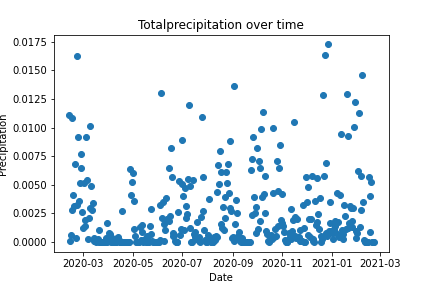
\includegraphics[width=.7\textwidth]{Figures/precipitation.png}


\subsection{Folium maps}
Furthermore, we created choropleths of hospitalized addition, population, and cases per capita based on the regions of the Netherlands. The figure below is a choropleth of cases per capita of the regions which illustrates that Rotterdam and the Hague were the most affected regions.



\includegraphics[width=.7\textwidth]{Figures/map.png}


\subsection{Pearson and Spearman correlation}
Moreover, we applied Pearson correlation to find the quantitative representations of the correlations between the corona data and weather variables, specifically between the cases per region and total precipitation variables. From our results, we were able to gather that the temperature above ground variable has the most statistical significance in regards to the p-value and also has the highest absolute value amongst the coefficients of all the weather variables used in the Pearson correlation test. On the other hand, total precipitation does not appear to have a significant correlation with corona outbreaks as shown by the Pearson correlation coefficient.

Likewise, the Spearman correlation test showed us similar results, i.e., temperature above ground has the highest absolute value of coefficient along with the lowest p-value indicating high statistical significance once again. In fact, the p-value is 0.0 which is exceptionally good, indicating that the null hypothesis is entirely rejected, which could either be a coincidence or a computational mistake. The coefficient has also increased relatively indicating a stronger correlation between the variables. The absolute value of Spearman's correlation coefficient of the total precipitation decreased to 0.073 compared to Pearson's correlation coefficient of 0.077, whereas the p-value increased indicating a decrease in statistical significance. The negative coefficient indicates a decreasing monotonic trend between corona cases per region and total precipitation.

The results gathered from the Bonferroni and Holm-Bonferroni corrections returned true for total precipitation which implies that the p values are below the threshold of 0.005 further indicating that total precipitation is statistically significant with regards to the corona outbreak intensity.

\subsection{OLS regression results}
In addition, we also performed Ordinary Least Squares (OLS) regression on our dataset. We used cases per region as our dependent variable and the weather variables as our independent variables. The result showed us that total precipitation had the highest coefficient of 0.0001 and a relatively low standard error. Moreover, we also looked at the logged OLS regression and found exactly the same results for the same variables.

\subsection{OLS regression of dataframe merged with stringency index data}
For the OLS merged with the stringency index, the total precipitation has a coefficient of 1.907e-06 which is relatively high compared to the other weather factors. However, it also has a quite high standard error of 3e-05. The lowest coefficient is -7.163e-17 for the “International Support” factor. The highest coefficient is international travel controls with the value 7.047e-06.